Bei der Analyse elektronischer Schaltungen geht man in der Regel so vor, dass in einem ersten Schritt die realen Bauelemente durch einfache Ersatzschaltbilder ersetzt werden. 
\section{Definitionen}
Unter einem \textbf{Zweipol} versteht man ein Bauelement mit zwei Anschlussklemmen. Für die Behandlung von Zweipolen in den Netzwerken ist nur noch ihr \textbf{Klemmenverhalten}, also der Zusammenhang zwischen Strom und Spannung am betreffenden Bauelement, von Interesse, die praktische Realisierung durch eine dreidimensionale Anordnung und die ortsabhängige Verteilung der Feldgrössen spielen keine Rolle mehr. Die Beschreibung erfolgt durch einfache skalare Beziehungen zwischen den an den Klemmen zugänglichen Grössen Strom und Spannung.
\newline\newline
Durch die Zusammenschaltung von Bauelementen entstehen \textbf{elektrische Netzwerke}. Zur vollständigen Beschreibung eines Netzwerks muss neben dem Klemmenverhalten aller Komponenten auch die Verknüpfung der Bauelemente untereinander bekannt sein. Die Zusammenschaltung bezeichnet man als \textbf{Topologie}.
\newline\newline
Die grafische Darstellung von Netzwerken bezeichnet man als \textbf{Schaltbilder}. zur Darstellung der Bauelemente werden die Schaltsymbole verwendet. Die leitende Verbindung zwischen den Bauelementen wird als idealer Leiter angesehen und spielt bei der Schaltungsanalyse keine Rolle. Die einzelnen Verbindungen sollten möglichst geradlinig, kreuzungsfrei und ohne Richtungsänderungen dargestellt werden. Gleichzeitig sollte die Wirkungsrichtung bzw. die Signalflussrichtung den Normen entsprechend von links nach rechts oder von oben nach unten verlaufen.
\section{Zählpfeile}
Sei $U_{12}$ die elektrische Spannung als das Wegintegral der elektrischen Feldstärke
\begin{equation}
\boxed{U_{12}=\varphi_e\left(P_1\right)-\varphi_e\left(P_2\right)=\displaystyle \int_{P_1}^{P_2}\overrightarrow{E}\bullet \text{d}\overrightarrow{s}}
\end{equation}
Die beiden Indizes bei der Spannung verdeutlichen die Richtung, in der die Feldstärke integriert wird. Wendet man diese Beziehung auf die zylindrische Anordnung an, dann wird die Feldstärke von einem in der Äquipotentialfläche $\varphi_{e1}$ liegenden Punkt $P_1$ bis zu einem in der Äquipotentialfläche $\varphi_{e2}$ liegenden Punkt $P_2$, d.h. die Richtung der $x$-Koordinate integriert. Die Spannung wird dann ebenfalls in der gleichen Richtung positiv gezählt und in einem Schaltbild mit einem \textbf{Zählpfeil} versehen. Eine Kennzeichnung mit den Zahlen 1 und 2 ist dann nicht mehr notwendig. Ist der Wert der Spannung positiv, dann stimmt die Richtung des elektrischen Feldes mit der Integrationsrichtung und damit auch mit der \textbf{Zählrichtung für die Spannung} überein, der Pfeil zeigt von positiven zu negativen Ladungen.
\begin{figure}[H]
\frame{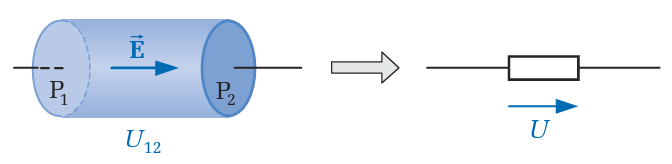
\includegraphics[scale=0.5]{../img/III/IIIa}}
\centering
\caption{Kennzeichnung der Spannung durch Zählpfeile.}
\label{fig_IIIa}
\end{figure}
\noindent Auf ähnlicher Weise wird ein Zählpfeil für den Strom vereinbart. Die Stromdichte erhält man durch die Bewegungsrichtung der positiven Ladungsträger. Den Strom erhält man, indem man das Skalarprodukt aus der gerichteten Stromdichte mit dem vektoriellen Flächenelement über die zu betrachtende Fläche integriert. Je nach Orientierung der vektoriellen Fläche ergeben sich unterschiedliche Vorzeichen für den Strom. Nach Festlegung der Richtung von $\text{d}\overrightarrow{A}$ kann dem Strom eindeutig ein Zählpfeil in diese Richtung zugeordnet werden. Besitzt der Strom $I$ einen positiven Wert, dann bewegen sich die positiven Ladungsträger in Richtung des vektoriellen Flächenelementes. 
\begin{figure}[H]
\frame{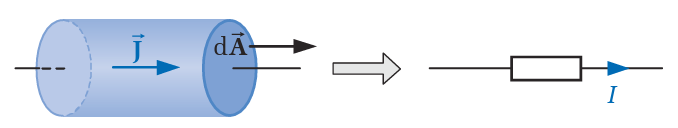
\includegraphics[scale=0.5]{../img/III/IIIb}}
\centering
\caption{Kennzeichnung des Stromes durch Zählpfeile.}
\label{fig_IIIb}
\end{figure}
\noindent Strom und Spannung sind skalare Grössen. Dennoch werden ihnen in Schaltungen Pfeile zugeordnet. Diese Pfeile dienen der Zählweise und dürfen nicht mit Vektoren verwechselt werden. Ein Spannungspfeil in Richtung der elektrischen Feldstärke zeigt positive Spannungen an. Ein Strompfeil in \textbf{Bewegungsrichtung der positiven Ladungsträger} zeigt positive Ströme an.
\section{Spannungs- und Stromquellen}
Zur Aufrechterhaltung eines Gleichstromes in einer Schatung müssen Quellen vorhanden sein, die die von den Elektroden abfliessenden Ladungsträger immer wieder nachliefern. Betrachte man zunächst zwei Ladungen $+Q$ und $-Q$ auf zwei Platten eines Kondensators. An den Kondensator wird ein Verbraucher, symbolisiert durch einen Widerstand, angeschlossen, an den die im Kondensator gespeicherte Energie abgegeben werden soll. Da die auf der negativ geladenen Platte befindlichen Elektronen durch die angeschlossenen Drähte und den Widerstand zur positiv geladenen Platte fliessen können, wird die anfänglich vorhandene Kondensatorspannung stetig abnehmen. Die aus dem Kondensator entnommene Energie wird im Widerstand in Wärme umgewandelt.
\begin{figure}[H]
\frame{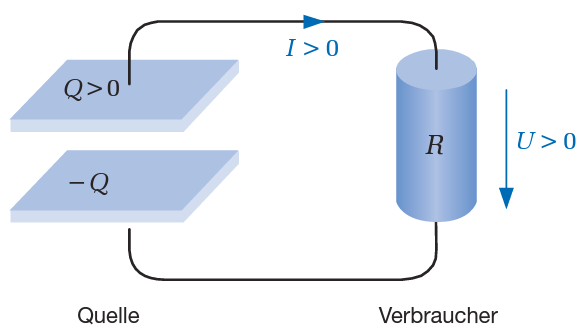
\includegraphics[scale=0.5]{../img/III/IIIc}}
\centering
\caption{Spannungsquelle und Verbraucher.}
\label{fig_IIIc}
\end{figure}
\noindent Der Kondensator in der vorliegenden Anordnung ist nur bedingt als Spannungsquelle einsetzbar. Einerseits nimmt seine Spannung zeitlich ab und andererseits kann er nur für einen begrenzten Zeitabschnitt Leistung abgeben, da lediglich die zuvor im elektrischen Feld zwischen den Kondensatorplatten gespeicherte Energie zur Verfügung steht. Der üblicherwese verwendete Begriff Quelle ist etwas irreführend, da keine Energieerzeugung, sondern immer nur Energieumwandlung stattfindet. In einem Akkumulator wird beispielsweise chemische Energie in elektrische Energie umgewandelt, im betrachteten Beispiel wird die elektrische Energie des Kondensators in Wärmeenergie am Widerstand umgewandelt.
\newline\newline  
Von einer \textbf{idealen Gleichspannungsquelle} wird jedoch erwartet, dass sie die Spannung unabhängig von dem Belastungswiderstand zeitlich konstant hält. Eine Batterie bzw. ein Akkumulator mit hinreichend grosser Energiereserve kommt dieser Situation schon sehr nahe. Mit elektronischen Schaltungen, die die vom 230V-Netz angebotene Energie in eine Gleichspannung  umwandeln, lassen sich nahezu ideale Spannungsquellen realisieren.
\newline\newline  
Für eine \textbf{ideale Spannungsquelle} gilt
\begin{enumerate}[$(i)$]
\item die Ausgangsspannung ist unabhängig von dem angeschlossenen Netzwerk.
\item der Strom hängt von dem angeschlossenen Netzwerk ab und stellt sich z.B. im Falle eines ohmschen Widerstandes entsprechend der Beziehung $I=U/R$ ein. 
\end{enumerate}
Für eine \textbf{ideale Stromquelle} gilt
\begin{enumerate}[$(i)$]
\item der Ausgangsstrom ist unabhängig von dem angeschlossenen Netzwerk.
\item die Ausgangsspannung hängt von dem angeschlossenen Netzwerk ab und stellt sich im Falle eines ohmschen Widerstandes entsprechend der Beziehung $U=RI$ ein. 
\end{enumerate}
\begin{figure}[H]
\frame{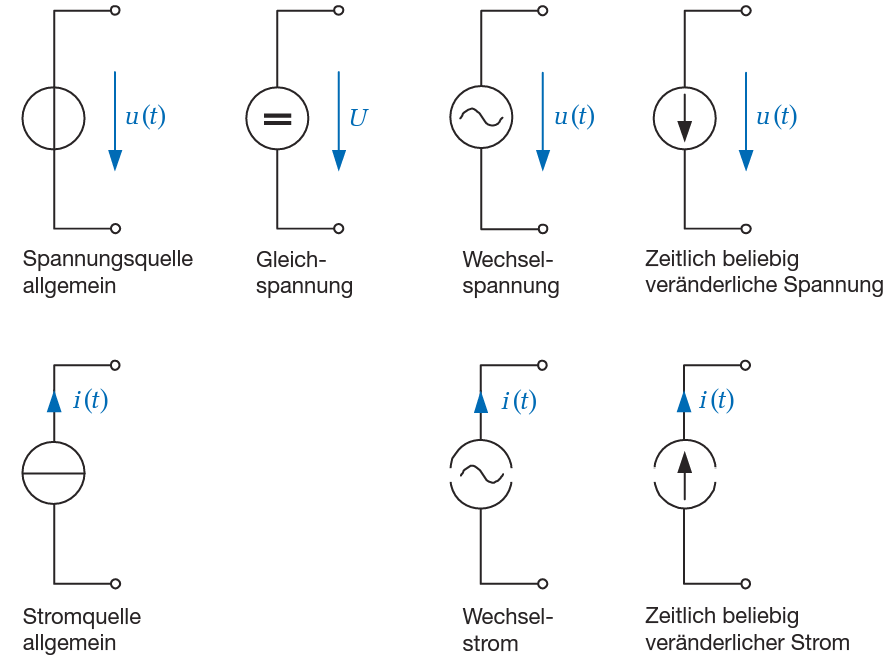
\includegraphics[scale=0.5]{../img/III/IIId}}
\centering
\caption{Ideale Spannungs- und Stromquellen.}
\label{fig_IIId}
\end{figure}
\section{Zählpfeilsysteme}
Ein Zählpfeilsystem am ohmschen Widerstand bei dem Strom und Spannung gleich gerichtet sind heisst \textbf{Verbraucherzählpfeilsystem}. Für $U>0$ wird der in die positive Anschlussklemme hineinfliessende Strom positiv gezählt. 
\newline\newline
Für die Quellen verwendet man üblichwerweise das \textbf{Generatorzählpfeilsystem}, bei dem Spannung und Strom entgegengesetzt gerichtet sind. Der aus der positiven Anschlussklemme herausfliessende Strom wird positiv gezählt. Diese Festlegung ist angepasst an den physikalischen Hintergrund, dass der Generator (Quelle) die Energie liefert, während der Verbraucher die Energie aufnimmt.
\begin{figure}[H]
\frame{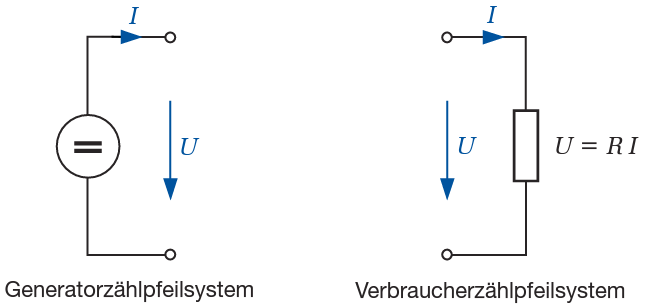
\includegraphics[scale=0.5]{../img/III/IIIe}}\quad
\frame{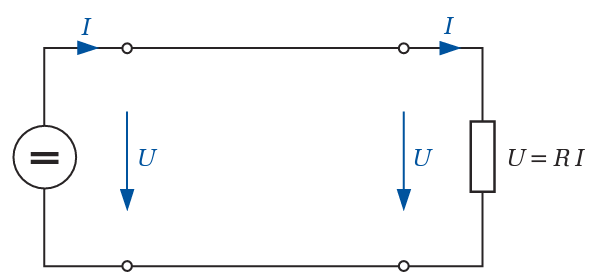
\includegraphics[scale=0.55]{../img/III/IIIj}}
\centering
\caption{Generator- und Verbraucherzählpfeilsystem.}
\label{fig_IIIe}
\end{figure}
\section{Die Kirchhoff'schen Gleichungen}
Eine der Hauptaufgaben der \textbf{Netzwerkanalyse} besteht darin, die Ströme und Spannungen an den einzelnen Zweipolen auszurechnen, sofern die verwendeten Netzwerkelemente (Widerstände, Kondensatoren, usw), ihre Verknüpfungen untereinander sowie die Quellen innerhalb des Netzwerkes bekannt sind. 
\newline\newline
Die schwarz ausgefüllten Markierungspunkte oder \textbf{Knoten} in dem Netzwerk zeigen an, dass die Leitungen an dieser Stelle elektrisch leitend miteinander verbunden sind, z.B. durch Zusammenschrauben oder Verlöten. Die Kreisringe markieren diejenigen Punkte im Netzwerk, zwischen denen die eingezeichnete Spannung gemessen wird.
\begin{figure}[H]
\frame{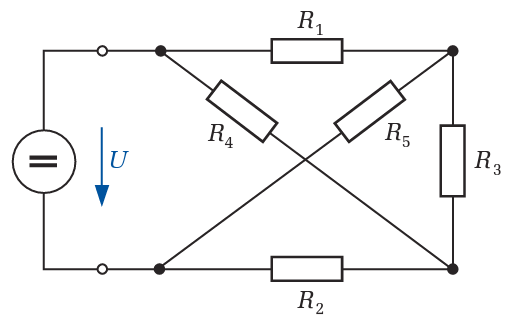
\includegraphics[scale=0.5]{../img/III/IIIf}}\quad 
\frame{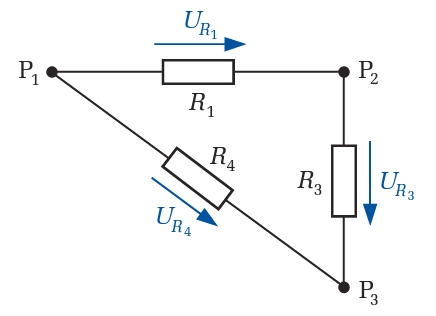
\includegraphics[scale=0.5]{../img/III/IIIg}}\quad 
\frame{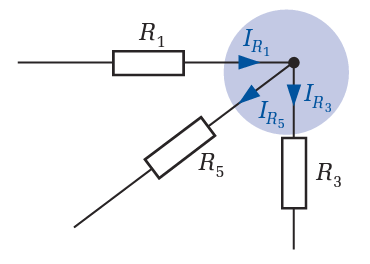
\includegraphics[scale=0.5]{../img/III/IIIh}}
\centering
\caption{Einfaches Netzwerk, Maschen- und Knotenregel.}
\label{fig_IIIf}
\end{figure}
\noindent Zur allgemeinen Netzwerkanalyse werden offenbar weitere Bestimmungsgleichungen benötigt. Einen ersten Zusammenhang erhält man aus dem Umlaufintegral der elektrischen Feldstärke, welches entlang eines geschlossenen Weges verschwinden muss. Zur Verdeutlichung dieses Zusammenhangs betrachtet man eine \textbf{Masche} in dargestellten Netzwerk.
\newline\newline
Nummeriert man die Verbindungspunkte gemäss einer Masche aus drei Punkte $P_1$, $P_2$ und $P_3$ mit drei Widerstände $R_1$, $R_2$ und $R_3$ des Netzwerkes, dann kann die Gleichung mit den \textbf{Feldstärken} folgendermassen geschrieben werden
\begin{equation}
\boxed{\displaystyle \oint_{C}\overrightarrow{E}\bullet \text{d}\overrightarrow{s}=\displaystyle \int_{P_1}^{P_2}\overrightarrow{E}\bullet \text{d}\overrightarrow{s}+\displaystyle \int_{P_2}^{P_3}\overrightarrow{E}\bullet \text{d}\overrightarrow{s}+\displaystyle \int_{P_3}^{P_1}\overrightarrow{E}\bullet \text{d}\overrightarrow{s}=\overrightarrow{0}}
\end{equation}
Diese Gleichung lässt sich mit den eingetragenen Spannungen und den ihnen willkürlich zugeordneten Zählpfeilen folgendermassen schreiben. 
\begin{equation}
\boxed{U_{R_1}+U_{R_3}-U_{R_4}=0}
\end{equation}
Verläuft der Integrationsweg $\text{d}\overrightarrow{s}$ entgegen der willkürlich angenommenen Zählrichtung bei der Spannung, dann ist diese mit negativen Vorzeichen einzusetzen. Dieser lässt sich als \textbf{Maschenregel} bezeichnen und lässt sich für jede geschlossene Masche in der allgemeinen Form darstellen. Die Summe aller Spannungen beim Umlauf in einer geschlossenen Masche ist Null. Spannungen, deren Zählpfeil in Umlaufrichtung verläuft, werden mit positivem Vorzeichen eingesetzt. 
\begin{equation}
\boxed{\displaystyle \sum_{\text{Masche}} U_{R_i}=0}
\end{equation}
Einen weiteren Zusammenhang erhält man aus dem Hüllflächenintegral der \textbf{Stromdichte}, das im stationären Strömungsfeld verschwindet.
\begin{equation}
\boxed{\displaystyle \oiint_{A}\overrightarrow{J}\bullet \text{d}\overrightarrow{A}=0}
\end{equation}
Zur Verdeutlichung dieses Zusammenhangs betrachtet man einen \textbf{Knoten} an einem Netzwerk. Die obige Gleichung besagt, dass im stationären zustand die Zahl der Ladungsträger innerhalb des markierten Bereiches zeitlich konstant sein muss, d.h. die Summe der zu dem Knoten hinfliessenden Ladungsträger muss gleich sein zu der Summe der vom Knoten wegfliessenden Ladungsträger.
\newline\newline
Dieser Sachverhalt lässt sich mit den Strömen und den ihnen zugeordneten Zählpfeilen folgendermassen schreiben
\begin{equation}
\boxed{I_{R_1}-I_{R_3}-I_{R_5}=0}
\end{equation}
\noindent Die Zählrichtung für die Ströme durch die Widerstände $R_1$ und $R_3$ am Knoten ist nicht mehr frei wählbar. Sie muss in Übereinstimmung mit den bereits festgelegten Zählpfeilen für die Spannungen entsprechend dem Verbraucherzählpfeilsystem festgelegt werden. Dieser lässt sich als \textbf{Knotenregel} bezeichnen und lässt sich für jeden Knoten in der allgemeinen Form darstellen. Die Summe aller zu einem Knoten hinfliessenden Ströme ist gleich der Summe aller von dem Knoten wegfliessenden Ströme.
\begin{equation}
\boxed{\displaystyle \sum_{\text{Knoten}}I_{R_i}=0}
\end{equation}
Der Begriff Knoten gilt nicht nur für die betrachtete leitende Verbindung zwischen den Drähten, sondern er schliesst die Möglichkeit ein, einzelne Netzwerkelemente oder auch grössere Teile einer Schaltung als Bestandteile des Knotens anzusehen. 
\begin{figure}[H]
\frame{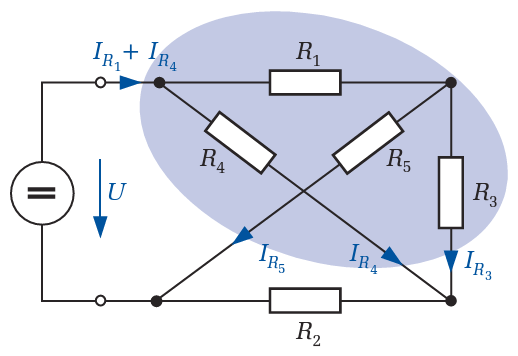
\includegraphics[scale=0.5]{../img/III/IIIi}}
\centering
\caption{Zur Verallgemeinerung des Begriffs Knoten.}
\label{fig_IIIi}
\end{figure}
\noindent Die Knotenregel bezieht sich in diesem Fall auf alle durch die Hüllfläche in Knoten hinein. bzw. aus dem Knoten herausfliessenden Ströme. Mit den definierten Ströme erhält man die identische Beziehung
\begin{equation} 
\boxed{I_{R_1}+I_{R_4}=I_{R_3}+I_{R_4}+I_{R_5}}
\end{equation} 
\section{Einfache Widerstandsnetzwerke}
Die Netzwerkanalyse kann dadurch vereinfacht werden, dass einzelne Teile eines Netzwerks vroab zusammengefasst werden. Dabei muss lediglich darauf geachtet werden, dass sich das Klemmenverhalten des neuen vereinfachten Netzwerks gegenüber dem ursprünglichen Netzwerk nicht ändert, d.h. beim Anlegen der gleichen Spannung an die Klemmen muss in beiden Fällen der gleiche Strom fliessen. An dieser Stelle werden die beiden Möglichkeiten der Reihenschaltung und Parallelschaltung von Widerständen untersucht. 
\newline\newline 
Bei der \textbf{Reihenschaltung} werden alle Widerstände von dem gleichen Strom durchflossen. Entsprechend dem Maschenumlauf setzt sich die gesamte an den Eingangsanschlüssen anliegende Spannung aus den Teilspannungen an den einzelnen Widerständen zusammen. Der Vergleich mit dem Netzwerk mit nur einem gesamtwiderstand liefert unmittelbar das Ergebnis
\begin{figure}[H]
\frame{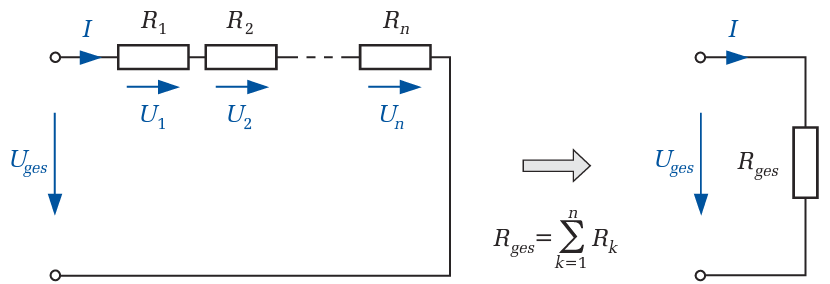
\includegraphics[scale=0.5]{../img/III/IIIk}}
\centering
\caption{Reihenschaltung von $n$ Widerständen.}
\label{fig_IIIk}
\end{figure}
\begin{equation}
\boxed{U_{\text{ges}}=\displaystyle \sum_{k=1}^{n}U_{k}=\displaystyle \sum_{k=1}^{n}\left(R_k\cdot I\right)=\left(\displaystyle \sum_{k=1}^{n}R_k\right)\cdot I =R_{\text{ges}}\cdot I}\quad \boxed{R_{\text{ges}}=\displaystyle \sum_{k=1}^nR_k}
\end{equation}
\noindent Bei der \textbf{Parallelschaltung} ist die Spannung an allen Widerständen gleich gross und der gesamte Eingangsstrom setzt sich aus den Strömen durch die einzelnen Widerstände zusammen. Bei der Parallelschaltung ist die Verwendung der Leitwerte sinnvoll. In diesem Fall liefert der Vergleich mit dem Ersatznetzwerk das Ergebnis
\begin{figure}[H]
\frame{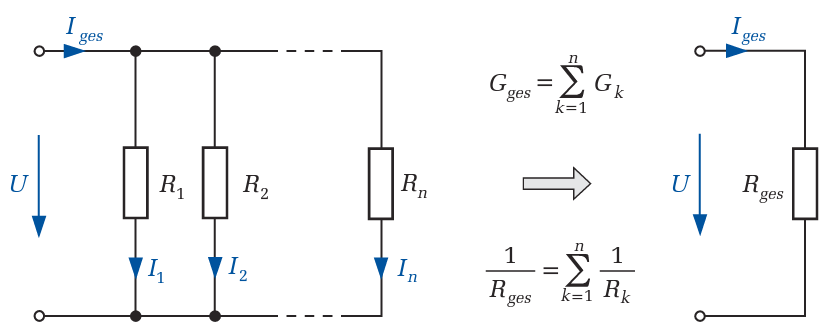
\includegraphics[scale=0.5]{../img/III/IIIl}}
\centering
\caption{Parallelschaltung von $n$ Widerständen.}
\label{fig_IIIl}
\end{figure}
\begin{equation}
\boxed{I_{\text{ges}}=\displaystyle \sum_{k=1}^nI_{ k}=\displaystyle \sum_{k=1}^n\left(\dfrac{U}{R_k}\right)=U\cdot \left(\displaystyle \sum_{k=1}^n\dfrac{1}{R_{k}}\right)=\dfrac{U}{R_{\text{ges}}}}\quad \boxed{\dfrac{1}{R_{\text{ges}}}=\displaystyle \sum_{k=1}^n\dfrac{1}{R_k}}\quad \boxed{G_{\text{ges}}=\displaystyle \sum_{k=1}^nG_k}
\end{equation}
Für den Sondernfall mit nur zwei parallel geschalteten Widerständen gilt dann
\begin{equation}
\boxed{R_{\text{ges}}=\dfrac{R_1R_2}{R_1+R_2}}
\end{equation}
Ein weiterer Sonderfall ist die Parallelschaltung von $n$ gleichen Widerständen. Der resultierende Gesamtwiderstand nimmt in diesem Fall den Wert an. 
\begin{equation}
\boxed{R_{\text{ges}}=\dfrac{R}{n}}
\end{equation}
Daraus ergeben sich folgende Merkmale:
\begin{enumerate}[$(a)$]
\item Bei der Reihenschaltung von Widerständen addieren sich die Werte der einzelnen Widerstände. 
\item Bei der Reihenschaltung ist der Gesamtwiderstand grösser als der grösste Einzelwiderstand.
\item Bei der Parallelschaltung berechnet sich der gesamte Leitwert aus der Summe der einzelnen Leitwerte.
\item Bei der Parallelschaltung ist der Gesamtwiderstand kleiner als der kleinste Einzelwiderstand.
\end{enumerate}
\subsection{Der Spannungsteiler - Reihenschaltung}
Die \textbf{Reihenschaltung} von zwei Widerständen kann benutzt werden, um eine gegebene Spannung $U$ mit hoherer Genauigkeit in kleinere Teilspannungen umzuwandeln. Für den fest eingestellten Spannungsteiler will man das Spannungsverhältnis $U_1/U_2$ sowie das Verhältnis von Ausgangsspannung zu Eingangsspannung $U_2/U$ bestimmen. 
\begin{figure}[H]
\frame{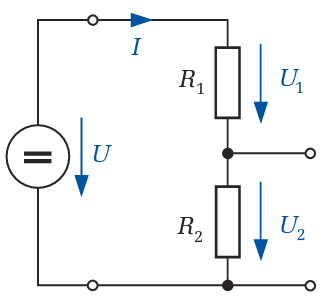
\includegraphics[scale=0.6]{../img/III/IIIm}}
\centering
\caption{Schaltung zur Spannungsteilung.}
\label{fig_IIIm}
\end{figure}
\noindent Somit besteht die Schaltung aus einer einzigen Masche, in der überall der gleiche Strom $I$ fliesst. Aus dem \textbf{Ohm'schen Gesetz} und mit der \textbf{Maschenregel} erhält man die Beziehungen
\begin{equation} 
\boxed{U_1=R_1I}\quad \boxed{U_2=R_2I}\quad \boxed{-U+U_1+U_2=0\Longrightarrow U=\left(R_1+R_2\right)I}
\end{equation} 
\begin{equation}
\boxed{\dfrac{U_1}{U_2}=\dfrac{R_1}{R_2}}\quad \boxed{\dfrac{U_2}{U}=\dfrac{U_2}{U_1+U_2}=\dfrac{R_2}{R_1+R_2}} 
\end{equation} 
Fliesst der gleiche Strom durch mehrere in Reihe geschaltete Widerstände, dann stehen die Teilspannungen im gleichen Verhältnis wie die Teilwiderstände, an denen sie abfallen. 
\newline\newline
Infolge des gleichen Stromes stehen die \textbf{Leistungen} an den Widerständen im gleichen Verhältnis zueinander wie die Spannungen und wie die Widerstände.
\begin{figure}[H]
\frame{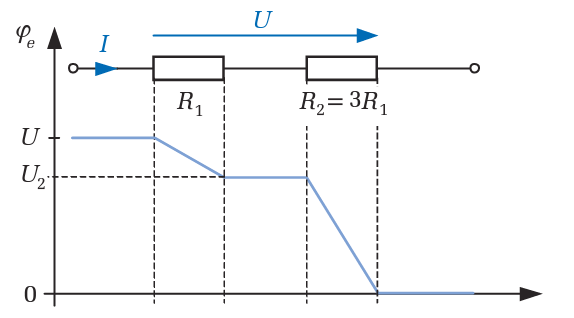
\includegraphics[scale=0.55]{../img/III/IIIn}}
\centering
\caption{Potentialverlauf an einer Reihenschaltung.}
\label{fig_IIIn}
\end{figure}
\noindent Die an einem Widerstand entstehende Teilspannung wird als \textbf{Spannungsabfall} bezeichnet. Definiert man das Potential am Minusanschluss der Spannungsquelle als Bezugswert $\varphi=0$, dann besitzt das Potential am positiven Anschluss den Wert $\varphi_e=U$. Mit einem ortsunabhängigen Feldstärkeverlauf innerhalb der Widerstände nimmt das Potential linear ab und man erhält entlang der Reihenschaltung für ein angenommenes Widerstandsverhältnis dargestellten Potentialverlauf.
\subsection{Der belastete Spannungsteiler}
\begin{figure}[H]
\frame{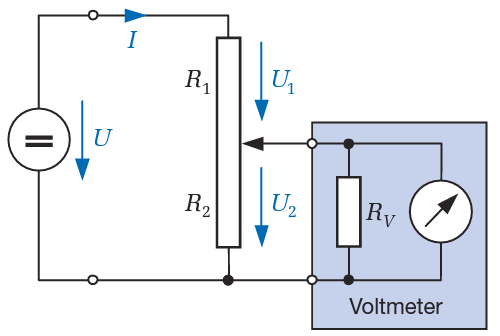
\includegraphics[scale=0.55]{../img/III/IIIo}}\quad
\frame{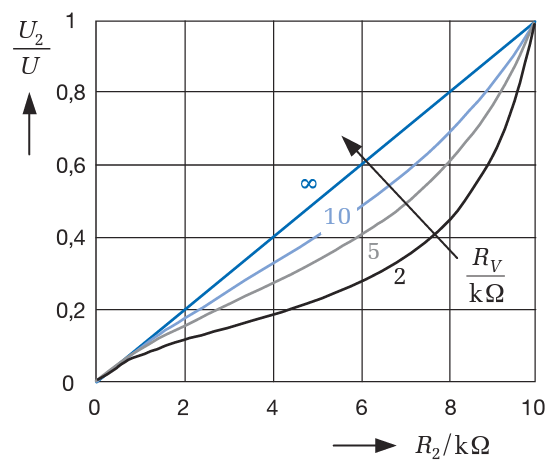
\includegraphics[scale=0.5]{../img/III/IIIp}}
\centering
\caption{\textbf{\textit{Links:}} Belasteter Spannungsteiler. \textbf{\textit{Rechts:}} Ausgangsspannung am belasteten Spannungsteiler für $R_1+R_2=10\text{k}\Omega$.}
\label{fig_IIIp}
\end{figure}
\noindent Die Spannung an dem Schleifkontakt eines Potentiometers soll mit einem realen Spannungsmessgerät (\textbf{Voltmeter}) gemessen werden. Dabei ist zu beachten, dass fast alle Spannungsmessgeräte von einem kleinen Strom durchflossen werden, der die in \textbf{Gleichung des Spannungsteilers} berechnete Spannungsteilung beeinflusst und das Messergebnis verfälscht. Diese Einfluss kann man erfassen, indem man das reale Messgerät durch ein ideales Messgerät mit unendlich grossem Innenwiderstand und zusätzlich durch einen parallel geschalteten Widerstand $R_V$ ersetzen.
\newline\newline 
Die Berechnung der resultierenden Spannung $U_2$ wird wesentlich vereinfacht, wenn man die Parallelschaltung der beiden Widerstände $R_2$ und $R_V$ durch einen neuen Widerstand $R_{\text{par}}$ ersetzen und die Spannung $U_2$ aus der Reihenschaltung von $R_1$ und $R_{\text{par}}$ bestimmen
\begin{equation}
\boxed{R_{\text{par}}=\dfrac{R_2R_V}{R_2+R_V} \Longrightarrow\dfrac{U_2}{U}=\dfrac{R_{\text{par}}}{R_1+R_{\text{par}}}=\dfrac{R_2R_V}{R_1\left(R_2+R_V\right)+R_2R_V}}
\end{equation}
\subsection{Messbereich eines Spannungsmessgerätes}
Ein Anwendungsbeispiel für den Spanungsteiler ist die Messbereichserweiterung eines Voltmeters. Soll mit dem Messgerät eine Spannung $U$ gemessen werden, die die maximal zulässige Spannung am Voltmeter $U_{\text{max}}$ überschreitet, dann kann die zu messende Spannung mit einem in Serie geschalteten Vorwiderstand $R_S$ heruntergeteilt werden. Der Wert des Vorwiderstandes kann mit Hilfe der \textbf{Gleichung des Spannungsteilers} berechnet werden
\begin{figure}[H]
\frame{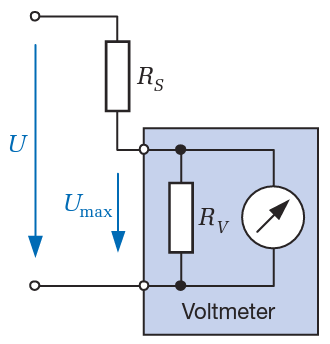
\includegraphics[scale=0.55]{../img/III/IIIq}}
\centering
\caption{Voltmeter mit Vorwiderstand.}
\label{fig_IIIq}
\end{figure}
\begin{equation}
\boxed{\dfrac{U_{\text{max}}}{U}=\dfrac{R_V}{R_S+R_V}\Longrightarrow R_S=\left(\dfrac{U}{U_{\text{max}}}-1\right)R_V}
\end{equation}
\subsection{Der Stromteiler - Parallelschaltung}
Zur Aufteilung eines Gesamtstromes in mehrere Teilströme werden Widerstände parallel geschaltet. Für eine Schaltung will man das Verhältnis $I_1/I_2$ sowie das Verhältnis von Ausgangsstrom zu Quellenstrom $I_2/I$ bestimmen. 
\begin{figure}[H]
\frame{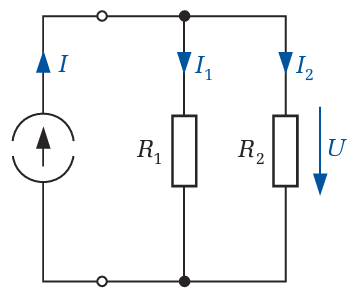
\includegraphics[scale=0.55]{../img/III/IIIr}}
\centering
\caption{Schaltung zur Stromleitung.}
\label{fig_IIIr}
\end{figure}
\noindent Mit der gleichen Spannung an den beiden parallel ligenden Widerständen gelten nach dem \textbf{Ohm'schen Gesetz} und mit der \textbf{Knotenregel} die Beziehungen
\begin{equation}
\boxed{I_1=\dfrac{U}{R_1}}\quad \boxed{I_2=\dfrac{U}{R_2}}\quad \boxed{-I+I_1+I_2=0\Longrightarrow I=U\left(\dfrac{1}{R_1}+\dfrac{1}{R_2}\right)=U\dfrac{R_1+R_2}{R_1R_2}}
\end{equation}
\begin{equation}
\boxed{\dfrac{I_1}{I_2}=\dfrac{R_2}{R_1}=\dfrac{G_1}{G_2}}\quad \boxed{\dfrac{I_2}{I}=\dfrac{R_1}{R_1+R_2}=\dfrac{G_2}{G_1+G_2}}
\end{equation}
Liegt die gleiche Spannung an mehreren parallel geschalteten Widerständen, dann stehen die Ströme im gleichen Verhältnis wie die Leitwerte, die sie durchfliessen. Die \textbf{Leistungen} an den Widerständen verhalten sich wegen der gleichen Spannung wie die Ströme durch die Widerstände und stehen im gleichen Verhältnis wie die Leitwerte.
\subsection{Messbereich eines Strommessgerätes}
Zur Messung eines Stromes wird das Messgerät (\textbf{Ampèremeter}) in den Strompfad geschaltet, sein Innenwiderstand $R_A$ sollte daher möglichst gering sein, um das Messergebnis nur wenig zu beeinflussen. Soll ein Strom gemessen werden, der den maximal zulässigen Bereich des Ampèremeters $I_{\text{max}}$ überschreitet, dann kann der Gesamtstrom $I$ durch einen parallel geschalteten Widerstand heruntergeteilt werden. Der Wert des Parallelwiderstandes kann mit Hilfe der \textbf{Gleichung des Stromleiters} berechnet werden.
\begin{figure}[H]
\frame{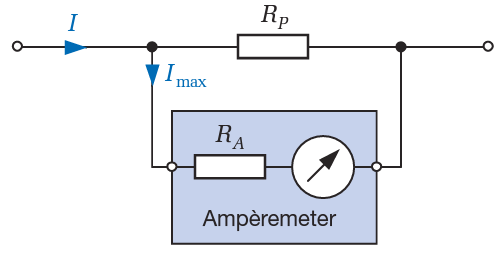
\includegraphics[scale=0.55]{../img/III/IIIs}}
\centering
\caption{Ampèremeter mit Parallelwiderstand.}
\label{fig_IIIs}
\end{figure}
\begin{equation}
\boxed{\dfrac{I_{\text{max}}}{I}=\dfrac{R_p}{R_p+R_A}\longrightarrow R_p=\dfrac{I_{\text{max}}}{I-I_{\text{max}}}R_A}
\end{equation}
\subsection{Widerstandsmessung}
\begin{figure}[H]
\frame{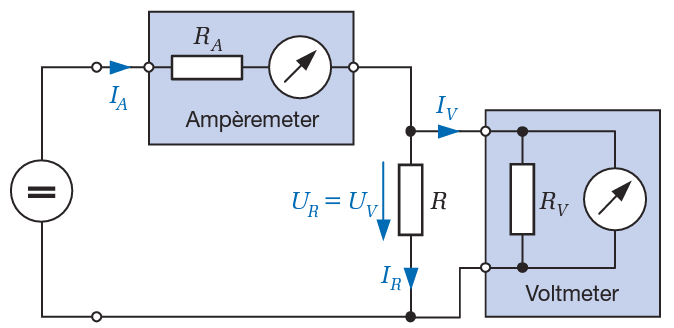
\includegraphics[scale=0.55]{../img/III/IIIt}}
\centering
\caption{Korrekte Spannungsmessung.}
\label{fig_IIIt}
\end{figure}
\noindent Bei der Schaltung der \textbf{\textit{Abbildung \ref{fig_IIIt}}} wird die Spannung am Widerstand richtig erfasst, das Ampèremeter misst allerdings nicht nur den Strom $I_R$ durch den Widerstand, sondern zusätzlich auch noch den Strom $I_V$ durch das Voltmeter. Für den Widerstandswert $R$ erhält man 
\begin{equation}
\boxed{R=\dfrac{U_R}{I_R}=\dfrac{U_V}{I_A-I_V}=\dfrac{U_V}{I_A-U_V/R_V}=\dfrac{U_VR_V}{I_AR_V-U_V}}
\end{equation}
\noindent Der Innenwiderstand des Ampèremeters spielt bei dieser Messanordnung keine Rolle. Im Falle eines idealen Voltmeters $R_V\rightarrow \infty$ vereinfacht sich die obige Gleichung auf den Zusammenhang $R=U_V/I_A$, d.h. der Wert $R$ kann direkt aus den beiden Messwerten berechnet werden.
\begin{figure}[H]
\frame{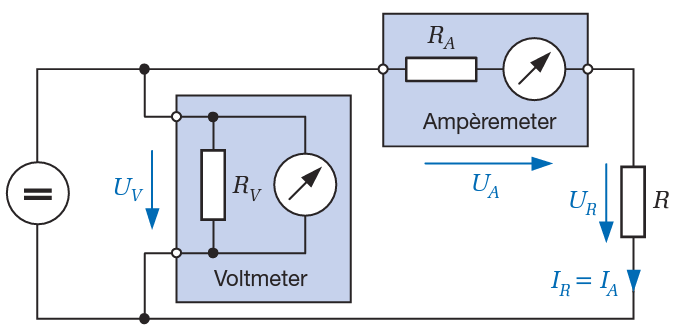
\includegraphics[scale=0.55]{../img/III/IIIu}}
\centering
\caption{Korrekte Strommessung.}
\label{fig_IIIu}
\end{figure}
\noindent Bei der alternativen Messanordnung wird der Strom durch den Widerstand richtig gemessen, allerdings wird jetzt der Spannungsabfall $U_A$ am Innenwiderstand des Ampèremeters bei der Spannungsmessung miterfasst. Den Widerstandswert erhält man aus der Beziehung
\begin{equation}
\boxed{R=\dfrac{U_R}{I_R}=\dfrac{U_V-U_A}{I_A}=\dfrac{U_V-R_AI_A}{I_A}}
\end{equation}
In diesem Fall spielt der Innenwiderstand des Voltmeters keine Rolle. Im Falle eines idealen Ampèremeters $R_A\rightarrow 0$ vereinfacht sich die obige Gleichung auf den Zusammenhang $R=U_V/I_A$, d.h. der Wert $R$ kann wieder direkt aus den beiden Messwerten berechnet werden.
\newline\newline
Allgemein stellt man sich die Aufgabe, den ohmschen Widerstand $R$ eines Bauteils durch gleichzeitige Strom- und Spannungsmessung und mit Hilfe des Ohm'schen Gesetzes zu bestimmen. Da das Ampèremeter den Strom durch den Widerstand messen soll, muss es in Reihe zum Widerstand geschaltet werden. Zur erfassung der Spannung am Widerstand muss das Voltmeter aber parallel zum Widerstand angeschlossen werden. 
\section{Reale Spannungs- und Stromquellen}
Wird eine Spannungsquelle durch einen Verbraucher belastet, dann ruft der Strom innerhalb der Quelle, z.B. an den internen Anschlussleistungen einen Spannungsabfall und damit Verluste hervor. Dieser Einfluss wird durch einen zur \textbf{idealen Quellenspannung} $U_0$ in Reihe liegenden Innenwiderstand $R_i$ erfasst. In der Praxis kann die Beschreibung des Quellenverhaltens durch Ersatznetzwerke noch wesentlich komplizierter werden, insbesondere wenn zeitabhängige Ströme und Spannungen betrachtet werden.
\newline\newline
Die Berücksichtigung der Verlustmechanismen führt auf das dargestellte einfache \textbf{Ersatzschaltbild einer Spannungsquelle}. Wird kein Verbraucher angeschlossen, dann fliesst kein Strom und die an den Anschlussklemmen vorliegende Spannung $U=U_L=U_0$ wird als \textbf{Leerlaufspannung} $U_L$ (=Quellenspannung) bezeichnet.
\begin{figure}[H]
\frame{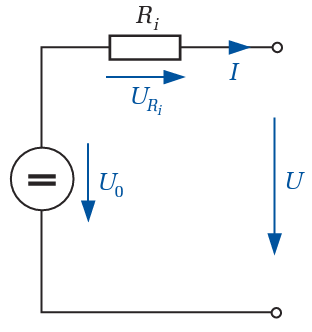
\includegraphics[scale=0.6]{../img/III/IIIv}}
\centering
\caption{Spannungsquelle mit Innenwiderstand.}
\label{fig_IIIv}
\end{figure}
\noindent Verbindet man die beiden Anschlussklemmen miteinander (\textbf{Kurzschluss}), dann wird der \textbf{Kurzschlussstrom} nur durch den Innenwiderstand begrenzt. 
\begin{equation}
\boxed{I_K=\dfrac{U_0}{R_i}}
\end{equation}
\noindent Die gesamte von der Quelle abgegebene Energie wird in diesem Fall am Innenwiderstand in Wärme umgewandelt, d.h. Spannungsquellen sollten nicht im Kurzschluss betrieben werden. Die Spannungsquelle wird durch Angabe von Leerlaufspannung $U_L=U_0$ und Innenwiderstand $R_i$ oder durch Angabe von Leerlaufspannung $U_L=U_0$ und Kurzschlussstrom $I_K$ eindeutig beschrieben.
\newline\newline
Ein geladener \textbf{Kondensator}, der seine Energie an einem Widerstand abgibt, verhält sich prinzipiell wie eine \textbf{Spannungsquelle}. Der Wert der Spannung ist durch die im Kondensator gespeicherte elektrische Energie gegeben und der Strom durch einen angeschlossenen Widerstand stellt sich in Abhängigkeit von dem Wert des Widerstandes ein.
\newline\newline
Im Gegensatz dazu hat die \textbf{Spule} einen gleichen Verhalten wie die von einer \textbf{Stromquelle}. In diesem Fall wird der Strom durch die magnetische Energie in der Spuile bestimmt und die Spannung stellt sich in Abhängigkeit von dem Wert eines angeschlossenen Widerstandes entsprechend dem Ohm'schen Gesetz ein.
\newline\newline
Die \textbf{\textit{Abbildung \ref{fig_IIIw}}} zeigt eine \textbf{Stromquelle} mit dem \textbf{Quellenstrom} $I_0$ und dem Innenwiderstand $R_i$. Da der Strom vorgegeben ist, muss immer ein geschlossener Strompfad vorhanden sein. Bei geöffneten Anschlussklemmen fliesst der gesamte Strom $I_0$ durch den parallel zur Quelle liegenden Innenwiderstand und die von der Quelle abgegebene Energie wird an $R_i$ in Wärme umgewandelt, d.h. Stromquellen sollten nicht im Leerlauf betrieben werden. 
\begin{figure}[H]
\frame{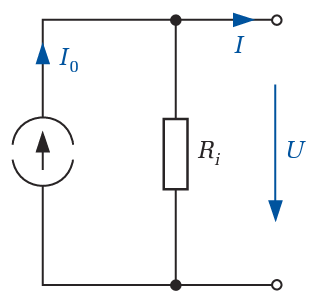
\includegraphics[scale=0.6]{../img/III/IIIw}}
\centering
\caption{Stromquelle mit Innenwiderstand.}
\label{fig_IIIw}
\end{figure}
\noindent Der an den Anschlussklemmen im Kurzschlussbetrieb zur Verfügung stehende Strom $I=I_K=I_0$ wird als \textbf{Kurzschlussstrom} $I_K$ (=Quellenstrom) bezeichnet.
\newline\newline
Für die \textbf{Leerlaufspannung} gilt
\begin{equation}
\boxed{U_L=I_0\cdot R_i}
\end{equation}
Bezüglich ihres Klemmenverhaltens können Spannungs- und Stromquelle ineinander umgerechnet werden. Dazu muss sichergestellt werden, dass beide Quellen die gleiche Leerlaufspannung und den gleichen Kurzschlussstrom aufweisen. Beide Forderungen werden erfüllt, wenn der Zusammenhang
\begin{equation}
\boxed{U_0=I_0\cdot R_i}
\end{equation}
zwischen Quellenstrom und Quellenspannung gilt. Unter dieser Voraussetzung verhalten sich beide Quellen bezüglich ihrer Anschlussklemmen gleich und der Strom $I$ durch einen beliebigen Verbraucher $R$ hat in beiden Fällen den gleichen Wert $I=U_0/\left(R+R_i\right)$. Das Ergebnis lässt sich mit den beiden äquivalenten Schaltungen in \textbf{\textit{Abbildung \ref{fig_IIIx}}} leicht bestätigen.
\begin{figure}[H]
\frame{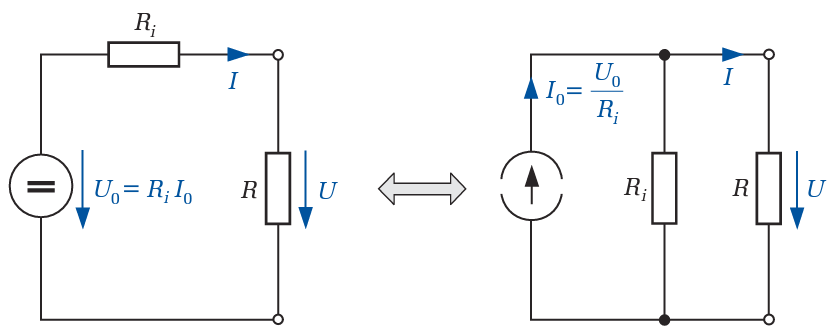
\includegraphics[scale=0.55]{../img/III/IIIx}}
\centering
\caption{Äquivalente Quellen.}
\label{fig_IIIx}
\end{figure}
\noindent An dieser Stelle ist noch ein Hinweis in Bezug auf die beiden Quellen angebracht. Obwohl an einen beliebigen Widerstand $R$ in beiden Fällen die gleiche Leistung abgegeben wird, ist das interne Verhalten der Quellen unterschiedlich. Die Ursache liegt an der unterschiedlichen Verlustleistung an dem jeweiligen Innenwiderstand $R_i$. Im Leerlauffall wird der Spannungsquelle keine Leistung entnommen, während die Stromquelle die Leistung $U_0I_0$ an $R_i$ abgibt. Im Kurzanschlussfall ist die Situation genau umgekehrt.
\section{Wechselwirkungen zwischen Quelle und Verbraucher}
Die Zusammenschaltung von Quellen und Verbrauchern wirft naturgemäss einige Fragen auf. In den folgenden Abschnitten werden die Besonderheiten bei der Verwendung mehrerer Quellen betrachtet und die Fragen nach der maximal von einer Quelle zur Verfügung gestellten Leistung sowie nach dem Wirkungsgrad beantwortet.
\subsection{Zusammenschaltung von Spannungsquellen}
In vielen Anwendungen findet man Reihenschaltungen von Spannungsquellen zur \textbf{Erhöhung der Gesamtspannung} oder auch Parallelschaltungen zur \textbf{Erhöhung des verfügbaren Stromes} oder zur Erhöhung der Kapazität, z.B. um einen Verbraucher über einen längeren Zeitraum mit Energie versorgen zu können.
\begin{figure}[H]
\frame{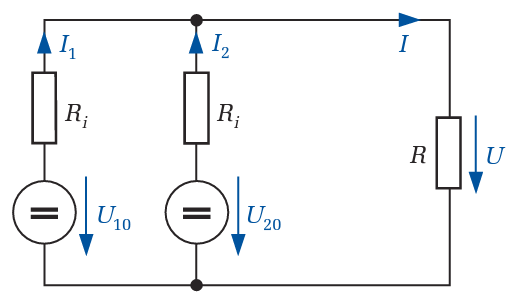
\includegraphics[scale=0.6]{../img/III/IIIy}}
\centering
\caption{Parallel geschaltete Spannungsquellen.}
\label{fig_IIIy}
\end{figure}
\noindent Die damit zusammenhängenden Probleme will man diskutieren anhand einer Schaltung mit zwei Spannungsquellen mit den gleichen Innenwiderständen $R_i$, aber mit unterschiedlichem Ladezustand. Aus den beiden parallel geschalteten Quellen mit den Leerlaufspannungen $U_{10}$ und $U_{20}$ soll ein Verbraucher $R$ mit Energie versorgt werden. Aus den Kirchhoff'schen Gleichungen folgt
\begin{equation}
\boxed{U\stackrel{!}{=}RI=R\left(I_1+I_2\right)\stackrel{!}{=}U_{10}-R_iI_1\stackrel{!}{=}U_{20}-R_iI_2}
\end{equation}
\begin{equation}
\boxed{I_1=\dfrac{1}{R_i^2+2RR_i}\Big[\left(R_i+R\right)U_{10}-RU_{20}\Big]}
\quad
\boxed{I_2=\dfrac{1}{R_i^2+2RR_i}\Big[\left(R_i+R\right)U_{20}-RU_{10}\Big]}
\end{equation}
Setzt man positive Werte für $U_{10}$, $U_{20}$, $R_i$ und $R$ ein, so ergibt sich eine positive Zahl für $I_1$ und eine negative Zahl für $I_2$. Infolge der unterschiedlichen Leerlaufspannungen wird in dem betrachteten Netzwerk die Quelle 2 zum Verbraucher. Die aus der Spannungsquelle $U_{10}$ entnommene Energie wird teilweise an den Widerstand $R$ abgegeben und teilweise zum Nachladen der zweiten Spannungsquelle $U_{20}$ verwendet. Eine gleicgmässig aufgeteilte Energieabgabe ist nur möglich bei identischen Quellen.
\begin{enumerate}[$(a)$]
\item Die Leistungsabgabe von parallel geschalteten Spannungsquellen ist unterschiedlich, wenn die Leerlaufspannungen oder die Innenwiderstände unterschiedlich sind.
\item In einem netzwerk mit mehreren Quellen kann ein Teil der Quellen als Verbraucher wirken, wenn sie nämlich die von anderen Quellen abgegebene Energie aufnehmen. Dieser Zustand ist gewollt beim Nachladen einer Batterie. 
\end{enumerate}
\subsection{Leistungsanpassung}
Eine weitere wichtige Frage im Zusammenwirken von Quelle und Verbraucher ist die Frage nach der maximal von einer Quelle zur Verfügung gestellten Leistung. Ausgehend von der Schaltung der \textbf{\textit{Abbildung \ref{fig_IIIz}}}, in der ein Verbraucher (Lastwiderstand) $R_L$ an eine durch die Leerlaufspannung $U_0$ und den Innenwiderstand $R_i$ charakterisierte Spannungsquelle angeschlossen ist, soll die Bedingung für maximale Leistungsabgabe an den Verbraucher abgeleitet werden.
\begin{figure}[H]
\frame{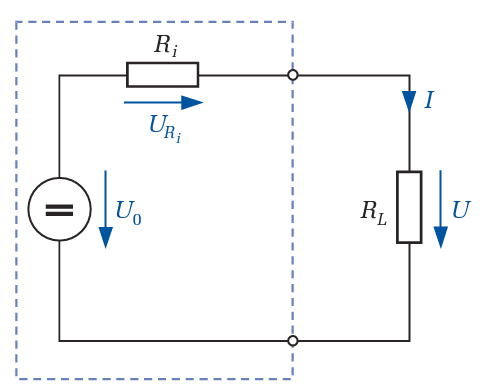
\includegraphics[scale=0.6]{../img/III/IIIz}}
\centering
\caption{Berechnung der maximalen Ausgangsleistung.}
\label{fig_IIIz}
\end{figure}
\noindent Gesucht ist also derjenige Wert für $R_L$, für den die Leistung $P_L$ an diesem Verbraucher den Maximalwert erreicht. Für die Leistung gilt
\begin{equation} 
\boxed{U-U_0+U_{R_i}=0\Longrightarrow U_0=U+U_{R_i}=I\left(R_L+R_i\right)}\quad \boxed{I=\dfrac{U_0}{R_i+R_L}}
\end{equation} 
\begin{equation} 
\boxed{P_L\left(R_L\right)=I^2\cdot R_L=\left(\dfrac{U_0}{R_i+R_L}\right)^2\cdot R_L}
\end{equation} 
Die maximale Leistung in Abhängigkeit von dem Wert $R_L$ erhält man aus der Forderung nach dem Verschwinden der ersten Ableitung
\begin{equation}
\boxed{\dfrac{\text{d}}{\text{d}R_L}\Big[P_L\left(R_L\right)\Big]= \dfrac{\text{d}}{\text{d}R_L}\Big[\dfrac{U_0^2\cdot R_L}{\left(R_i+R_L\right)^2}\Big]=U_0^2\cdot \dfrac{R_i-R_L}{\left(R_i+R_L\right)^3}\stackrel{!}{=}0\Longrightarrow R_L=R_i}
\end{equation}
Eine Gleichspannungsquelle gibt die maximale Leistung bei Widerstandsanpassung
\begin{equation}
\boxed{R_L=R_i}
\end{equation}
Die maximale Ausgangsleistung (\textbf{verfügbare Leistung}) beträgt dann
\begin{equation}
\boxed{P_{L,\text{max}}\left(R_L=R_i\right)=\left(\dfrac{U_0}{R_i+R_L}\right)^2\cdot R_L=\left(\dfrac{U_0}{R_i+R_i}\right)^2\cdot R_i=\left(\dfrac{U_0}{2R_i}\right)^2\cdot R_i=\dfrac{U_0^2}{4R_i}}
\end{equation}
Das Verhältnis aus der an den Widerstand $R_L$ abgegebenen Leistung zu der verfügbaren Leistung ist für den gesamten Wertebereich zwischen Kurzschluss und Leerlauf $0\leq R_L\leq \infty$
\begin{equation}
\boxed{\dfrac{P_L}{P_{L,\text{max}}}=\dfrac{4R_iR_L}{\left(R_i+R_L\right)^2}=\dfrac{4R_L/R_i}{\left(1+R_L/R_i\right)^2}}
\end{equation}
Zur besseren Übersicht wird auf der Abszisse aber nicht der Wertebereich von $R_L$ zwischen Null und Unendlich aufgetragem. Das Ergebnis lässt sich nämlich anschaulicher darstellen, wenn der von der Quelle abgegebene Strom für die Achseneinteilung verwendet wird. Dieser Strom nimmt seinen Maximalwert im Kurzschlussfall, d.h. bei $R_L=0$ an. 
\begin{equation}
\boxed{I\left(R_L\right)=\dfrac{U_0}{R_i+R_L}}\quad \boxed{I_{\text{max}}\left(R_L=0\right)=\dfrac{U_0}{R_i}}
\end{equation}
Das Verhältnis der beiden Ströme ändert sich also von 0 auf 1, wenn sich der Lastwiderstand von Leerlauf ($R_L=\infty$) auf Kurzschluss ($R_L=0$) reduziert. 
\begin{equation}
\boxed{\dfrac{I}{I_{\text{max}}}=\dfrac{R_i}{R_i+R_L}=\dfrac{1}{1+R_L/R_i}}
\end{equation}
\begin{figure}[H]
\frame{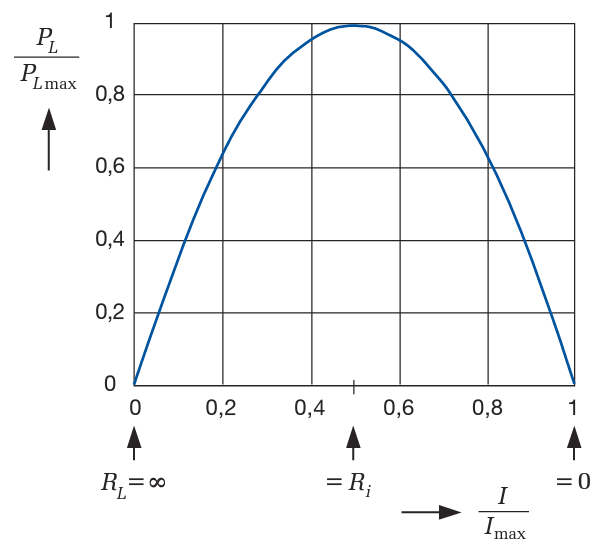
\includegraphics[scale=0.6]{../img/III/IIIaa}}
\centering
\caption{Normierte Ausgangsleistung als Funktion des normierten Stromes.}
\label{fig_IIIaa}
\end{figure}
\noindent Die Kurve in der \textbf{\textit{Abbildung \ref{fig_IIIaa}}} lässt sich leicht berechnen, indem für verschiedenen Zahlenverhältnisse $R_L/R_i$ mit der Abszissenwert und der jeweils zugehörige Ordinatenwert berechnet wird. Alternativ kann nach dem Widerstandsverhältnis $R_L/R_i$ aufgelöst und das Ergebnis eingesetzt werden. Damit erhält man direkt den gesuchten Zusammenhang
\begin{equation}
\boxed{\dfrac{P_L}{P_{L,\text{max}}}=\dfrac{4I}{I_{\text{max}}}\left(1-\dfrac{I}{I_{\text{max}}}\right)}
\end{equation}
Interessant sind die drei Zustände, Leerlauf, WIderstandsanpassung und Kurzschluss. Bei Widerstandsanpassung $R_L=R_i$ nimmt die Ausgangsleistung ihren Maximalwert $P_L=P_{L,\text{max}}$ an. Weicht der Widerstand $R_L$ von dem Wert $R_i$ ab, dann wird weniger Leistung von der Quelle an den Verbraucher abgegeben.An den beiden Grenzen Leerlauf und Kurzschluss verschwinden entweder Strom oder Spannung am Verbraucher, so dass die Leistung $P_L=UI$ ebenfalls in beiden Fällen verschwindet.
\subsection{Wirkungsgrad}
Mit kleiner werdendem Lastwiderstand in \textbf{\textit{Abbildung \ref{fig_IIIz}}} steigt der Strom kontinuerlich an. Obwohl die von der Quelle gelieferte Leistung 
\begin{equation}
\boxed{P_{\text{ges}}=U_0I\stackrel{!}{=}4\dfrac{P_{L,\text{max}}}{I_{\text{max}}}I\Longrightarrow \dfrac{P_{\text{ges}}}{P_{L,\text{max}}}=4\dfrac{I}{I_{\text{max}}}}
\end{equation}
damit ebenfalls ansteigt, nimmt die Leistung an Verbraucher in dem Bereich $R_L<R_i$ kontinuerlich ab. In der \textbf{\textit{Abbildung \ref{fig_IIIbb}}} sind sowohl die Verbraucherleistung $P_L$ als auch die von der Quelle abgegebene Leistung $P_{\text{ges}}$ mit dem gleichen Bezugswert $P_{L,\text{max}}$ dargestellt. Die Differenz zwischen den beiden Kurven entspricht der an dem Innenwiderstand der Quelle entstehenden Verlustleistung.
\begin{figure}[H]
\frame{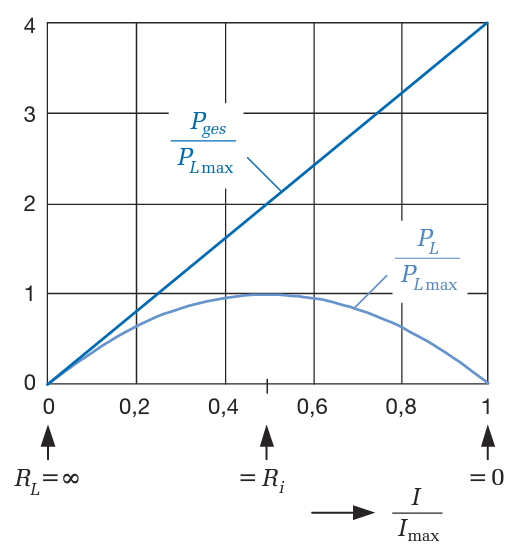
\includegraphics[scale=0.6]{../img/III/IIIbb}}\quad
\frame{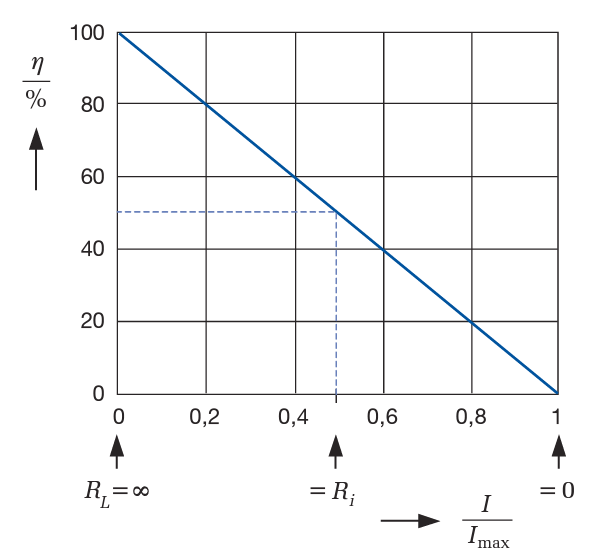
\includegraphics[scale=0.6]{../img/III/IIIcc}}
\centering
\caption{\textbf{\textit{Links:}} Von der Quelle abgegebene und vom Verbraucher aufgenommene Leistung.\textbf{\textit{Rechts:}} Wirkungsgrad.}
\label{fig_IIIbb}
\end{figure}
\noindent In diesem Zusammenhang stellt sich die Frage nach dem \textbf{Wirkungsgrad} $\eta$. Darunter versteht man das Verhältnis von der an dem Lastwiderstand verbrauchten Leistung zu der gesamten von der Quelle abgegebenen Leistung.
\begin{equation}
\boxed{\eta=\dfrac{P_L}{P_{\text{ges}}}\cdot 100\%=\dfrac{I^2R_L}{I^2\left(R_i+R_L\right)}\cdot 100\%=\dfrac{R_L/R_i}{1+R_L/R_i}\cdot 100\%=\left(1-\dfrac{I}{I_{\text{max}}}\right)\cdot 100\%}
\end{equation}
Aus dieser linearen abfallenden Funktion erkennt man, dass der Wirkungsgrad mit zunehmendem Strom aus der Quelle geringer wird. Bei Widerstandsanpassung beträgt der Wirkungsgrad nur 50\% , d.h. am Innenwiderstand der Quelle wird genau so viel Leistung verbraucht wie am Lastwiderstand.
\newline\newline
Die Wirkungsgradfrage ist von besonderem Interesse bei Energieübertragungssystemen. Die im Kraftwerk erzeugte Energie soll möglichst verlustarm zum Verbraucher transportiert werden. Bei vorgegebener Verbraucherleistung $P_L=UI$ und ebenfalls vorgegebenem Innenwiderstand $R_i$ lässt sich der Wirkungsgrad steigern, wenn der Strom möglichst klein und als Konsequenz die Spannung entsprechend gross wird. In der Praxis erfolgt die Energieübertragung auf Hochspannungsleistungen mit Spannungen im Bereich von einigen hundert kV.
\section{Das Überlagerungsprinzip}
Enthält eine Schaltung mehrere Quellen, dann können die Ströme und Spannungen in den einzelnen Zweigen des Netzwerks durch die Überlagerung von Teillösungen berechnet werden. Voraussetzung dafür ist, dass an den einzelnen Netzwerkelementen lineare Beziehungen zwischen Strom und Spannung gelten. Zur Berechnung einer Teillösung wird nur eine einzige Quelle betrachtet, die anderen Quellen werden zu Null gesetzt. Für diese Quelle wird dann die Netzwerkanalyse durchgeführt, d.h. es werden die Ströme und Spannungen in den interessierenden Zweigen berechnet. 
\newline\newline
Bei dieser Vorgehensweise muss sichergestellt werden, dass nach der Überlagerung der Teillösungen in jedem Zweig, der eine Stromquelle enthält, genau der vorgegebene Quellenstrom fliesst und dass in jedem Zweig mit einer Spannungsquelle genau die vorgegebene Spannung vorliegt. Bei der Überlagerung dürfen keine zusätzlichen Ströme zu einer Stromquelle und keine zusätzliche Spannungen zu einer Spannungsquelle addiert werden. Nullsetzen der Quellen bedeutet also, dass eine Spannungsquelle durch einen Kurzschluss (keine Spannung in dem Zweig, d.h. $U=0$) und eine Stromquelle durch einen Leerlauf (kein Strom in dem Zweig, d.h. $I=0$) ersetzt wird.
\newline\newline
Ist die Netzwerkanalyse in dieser Weise für jede Quelle einzeln durchgeführt, dann ist der gesamte Strom in einem Zweig des Netzwerks bei Vorhandensein aller Quellen gleich der Summe aller vorher berechneten Teilströme in diesem Zweig.
\newline\newline
Betrachte man folgendes Netzwerk in der \textbf{\textit{Abbildung \ref{fig_IIIdd} Links}} mit jeweils einer Strom- und einer Spannungsquelle. Mit der beschriebene Methode will man den Strom $I_2$ durch den Widerstand $R_2$ berechnen.
\begin{figure}[H]
\frame{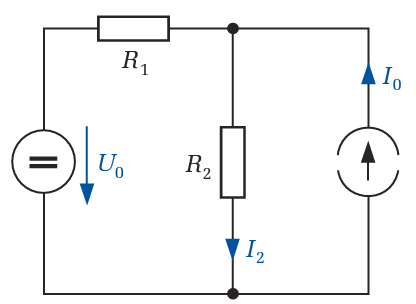
\includegraphics[scale=0.6]{../img/III/IIIdd}}\quad 
\frame{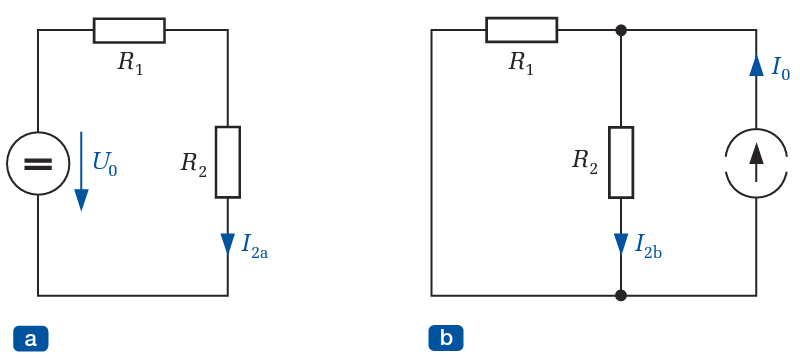
\includegraphics[scale=0.6]{../img/III/IIIee}}
\centering
\caption{\textbf{\textit{Links:}} Überlagerung von Quellen. \textbf{\textit{Rechts:}} Netzwerke für die beiden Lösungen}
\label{fig_IIIdd}
\end{figure}
\noindent In der \textbf{ersten Teillösung} soll der Beitrag der Spannungsquelle $U_0$ zum gesuchten Strom berechnet werden. Wird die Stromquelle durch einen Leerlauf ersetzt, dann vereinfacht sich das Netzwerk wie in \textbf{\textit{Abbildung \ref{fig_IIIdd} Rechts a}} dargestellt. Der Strom $I_{2a}$ durch den Widerstand $R_2$ kann für diese Teillösung mit dem Ohm'schen Gesetz ummittelbar angegeben werden.
\begin{equation} 
\boxed{I_{2a}=\dfrac{U_0}{R_1+R_2}}
\end{equation} 
In der \textbf{zweiten Teillösung} wird nur die Stromquelle $I_0$ betrachtet, wobei die Spannungsquelle durch einen Kurzschluss ersetzt werden muss. Das resultierende Netzwerk in \textbf{\textit{Abbildung \ref{fig_IIIdd} Rechts b}} ist aber identisch zu dem Stromteiler, so dass der Strom durch $R_2$ ebenfalls direkt angegeben werden kann.
\begin{equation} 
\boxed{I_{2b}=\dfrac{R_1}{R_1+R_2}I_0}
\end{equation} 
Damit ist der \textbf{Gesamtstrom} für das Ausgangsnetzwerk in \textbf{\textit{Abbildung \ref{fig_IIIdd} Links}} bekannt.
\begin{equation}
\boxed{I_2=I_{2a}+I_{2b}=\dfrac{U_0+R_1I_0}{R_1+R_2}}
\end{equation}
Voraussetzung für die Überlagerung war ein linearer Zusammenhang zwischen Strom und Spannung an den Komponenten. Betrachtet man die Gleichung für die Leistung an dem Widerstand $R_2$, in der der Strom nicht mehr linear, sondern quadratisch vorkommt.
\begin{equation}  
\boxed{P_2=I_2^2R_2=\left(I_{2a}+I_{2b}\right)^2R_2=\left(I_{2a}^2+2I_{2a}I_{2b}+I_{2b}^2\right)^2R_2}
\end{equation}  
Bei linearer Überlagerung der einzelnen Beiträge fällt das gemischte Glied weg und man erhält ein falsches Ergebnis.
\begin{equation}
\boxed{P_{2a}+P_{2b}=I_{2a}^2R_2+I_{2b}^2R_2=P_2-2I_{2a}I_{2b}R_2\neq P_2}
\end{equation}
Wegen des nichtlinearen Zusammenhangs zwischen Strom und Leistung darf die Leistung an einem Widerstand nicht durch Summation der Teilleistungen infolge der Teilströme berechnet werden. 
\section{Analyse umfangreicher Netzwerke}
Umfangreicher Netzwerke können Spannungsquellen, Stromquellen und Widerstände enthalten. An allen im Netzwerk vorhandenen Widerständen sind Spannung und Strom proportional zueinander. Die Gleichungen zur Beschreibung der Netzwerke sind dann ebenfalls linear. Unabhängig von dieser Einschränkung gelten die folgenden Überlegungen allgemein auch für nichtlineare Netzwerke. Der Unterschied besteht lediglich in dem erhöhten mathematischen Aufwand bei der Auflösung der sich ergebenden nichtlinearen Gleichungssysteme.
\newline\newline
Ausgangspunkt für die weiteren Betrachtungen ist die Schaltung in der \textbf{\textit{Abbildung \ref{fig_IIIff}}}. Mit Hilfe des Ohm'schen Gesetztes können die Anzahl der Unbekannten auf die Anzahl der Zweipole reduziert werden. An jedem Widerstand bleibt entweder Spannung oder Strom unbestimmt, an einer Spannungsquelle ist der Strom unbekannt und an einer Stromquelle die Spannung. 
\begin{figure}[H]
\frame{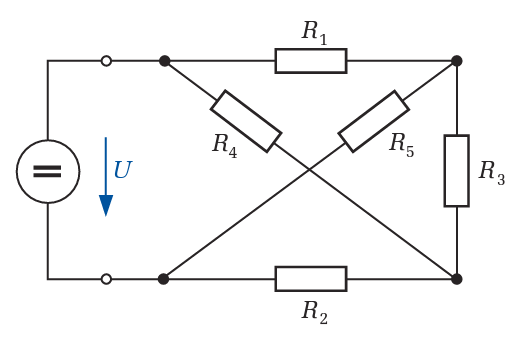
\includegraphics[scale=0.6]{../img/III/IIIff}}\quad
\frame{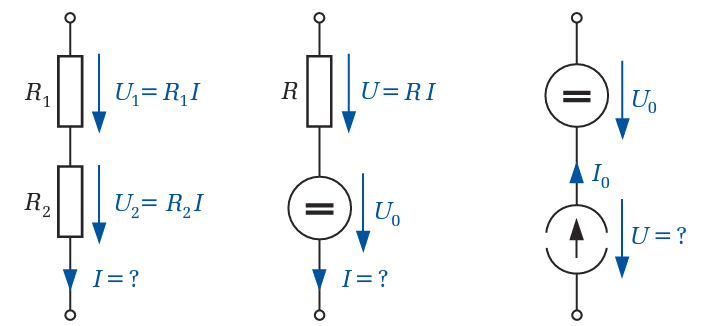
\includegraphics[scale=0.6]{../img/III/IIIgg}}
\centering
\caption{\textbf{\textit{Links:}} Einfaches Netzwerk. \textbf{\textit{Rechts:}} Zweipolnetzwerke.}
\label{fig_IIIff}
\end{figure}
\noindent In \textbf{\textit{Abbildung \ref{fig_IIIff} Rechts}} sind einige Beispiele für zusammengesetzte Zweipole dargestellt. Auch in diesen Fällen verbleibt immer genau eine Unbekannte. Ist beispielsweise der Strom im mittleren Zweipol bekannt, dann lässt sich daraus die Spannung am Widerstand berechnen. 
\newline\newline
Unabhängig von dem Aufbau der Zweipole kann man feststellen, dass ihre Anzahl in einem Netzwerk identisch ist mit der Anzahl der unbekannten Grössen. In der Netzwerktheorie spricht man allgemein von \textbf{Zweigen} und meint damit die beliebig zusammengesetzten Zweipole, die zwischen zwei Knoten des Netzwerkes liegen. 
\begin{enumerate}[$(i)$]
\item Unter Zuhilfenahme der an den Komponenten geltenden Beziehungen zwischen Strom und Spannung kann die Anzahl der unbekannten Ströme und Spannungen für jeden Zweig auf eine Unbekannte reduziert werden.
\item Setzt sich ein Netzwerk aus $z$ Zweigen zusammen, dann werden genau $z$ linear unabhängige Gleichungen zur Bestimmung der verbleibenden Unbekannten benötigt.
\item Zur Aufstellung der Gleichungen stehen die Kirchhoff'schen Sätze, nämlich die Maschenregel und die Knotenregel zur Verfügung.  
\end{enumerate}
\subsection{Darstellung des Netzwerkgraphen}
\begin{figure}[H]
\frame{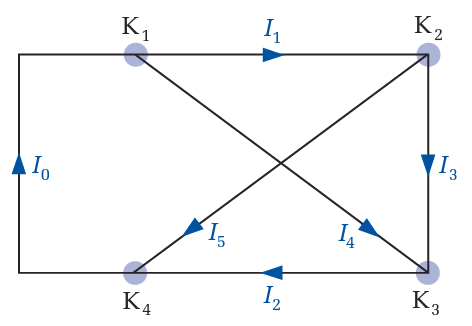
\includegraphics[scale=0.55]{../img/III/IIIhh}}
\centering
\caption{Netzwerkgraph.}
\label{fig_IIIhh}
\end{figure}
Das Netzwerk wird ohne die Komponenten nochmals dargestellt. In dieser als \textbf{Netzwerkgraph} bezeichneten Darstellung ist die Struktur des Netzwerks, d.h. welche Zweige an welchen Knoten miteinander verbunden sind, besonders gut zu erkennen.
\subsection{Festlegung der Zählrichtungen}
Für jeden Zweig ohne Quellen wird vereinbart, in welcher Richtung der Strom positiv gezählt werden soll. Diese Festlegung ist willkürlich und hat keinen Einfluss auf das Ergebnis, sie muss aber für die gesamte Analyse konsequent beibehalten werden. Die tatsächliche Stromrichtung ist erst nach Auflösung des Gleichungssystems bekannt. Hat der Strom einen positiven Wert, dann stimmt seine tatsächliche Richtung mit der gewählten Richtung überein, hat er dagegen einen negativen Wert, dann fliesst er entgegengesetzt zur gewählten Richtung. Die Zählrichtung für die Spannung wird am Verbraucher in Richtung des Stromes gewählt.
\newline\newline
Bei Spannungsquellen wird die Spannung, bei Stromquellen der Strom in der von der Quelle vorgegebenen Richtung gezählt. Die Richtung des Stromes bei einer Spannungsquelle und dir Richtung der Spannung bei einer Stromquelle können frei gewählt werden. Befindet sich nur eine Quelle in einem Zweig, dann empfiehlt sich die Verwendung des Generatorzählpfeilsystems.
\subsection{Aufstellung der Knotengleichungen}
Zur Vermeidung linear abhängiger Gleichungen betrachtet man üblicherweise nur Knoten in denen keine Komponenten enthalten sind. Unterschiedliche Knoten führen auf identische und damit linear abhängige Gleichungen. Das zu betrachtende Netzwerk besitzt vier Knoten. Da die Summe aller Ströme in allen Knoten immer Null ist, ist eine der Knotengleichungen linear von den anderen abhängig. Besitzt ein Netzwerk $k$ Knoten, dann können immer $k-1$ linear unabhängige Knotengleichungen aufgestellt werden. Die Auswahl des nicht zu berücksichtigenden Knotes hat keinen Einfluss auf das Ergebnis. Für das betrachtete Beispiel gilt
\begin{equation}
\boxed{\begin{array}{llllllll}
K_1:&I_0&-I_1&&&-I_4&&=0\\
K_2:&&I_1&&-I_3&&-I_5&=0\\
K_3:&&&-I_2&+I_3&+I_4&&=0\\
\end{array}}
\end{equation}
Die lineare Unabhängigkeit dieser Gleichungen erkennt man unmittelbar daran, dass in jeder Gleichung ein Strom enthalten ist, der in den anderen Gleichungen nicht auftritt. Auf der anderen Seite ist die lineare Abhängigkeit der Gleichung am Knoten leicht zu überprüfenm, da diese Gleichung identisch ist zur Summe der bereits angegebenen Gleichungen. 
\subsection{Aufstellung der Maschengleichungen}
Die Anzhal $m$ der noch benötigten unabhängige Maschengleichungen beträgt $m=z-\left(k-1\right)$. Im Beispiel sind es 3 unabhängige Maschengleichungen zu sehen. Während der Aufstellung der $k-1$ knotengleichungen völlig unproblematisch ist, müssen bei der Auswahl der Maschen bestimmte Vorgehensweisen eingehalten werden. Es gibt verschiedene Möglichkeiten, die Maschen so auszuwählen, dass die resultierenden Gleichungen zwangsläufig linear unabhängig sind. Die unterschiedlichen Methoden laufen im Prinzip darauf hinaus, sicherzustellen, dass in jeder Masche ein \textbf{Zweig} enthalten ist, der in keiner anderen Masche vorkommt.
\newline\newline
\noindent Die erste Methode wird als \textbf{vollständiger Baum} bezeichnet. Zunächst werden alle $k$ Netzwerkknoten entlang der Zweige so miteinander verbunden, dass keine geschlossene Masche entsteht. Bei $k$ Knoten werden genau $k-1$ Zweige für die Verbindungen benötigt. Die in \textbf{\textit{Abbildung \ref{fig_IIIii}}} zeigt nur zwei der Möglichkeiten, für das gegebene Netzwerk einen vollständigen Baum zu konstruieren. 
\begin{figure}[H]
\frame{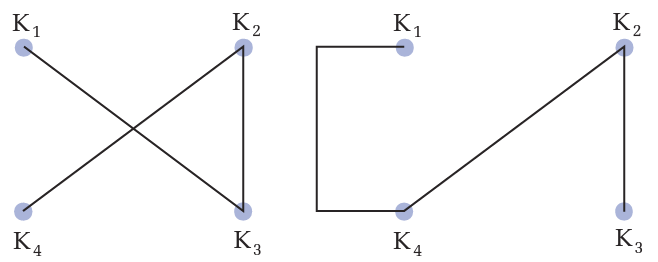
\includegraphics[scale=0.6]{../img/III/IIIii}}
\centering
\caption{Vollständiger Baum.}
\label{fig_IIIii}
\end{figure}
\noindent Von den insgesamt $z$ Zweigen des Netzwerkes gehören damit $k-1$ Zweige zu dem vollständigen Baum und $z-\left(k-1\right)=m$ Zweige, die so genannten \textbf{Verbindungszweige}, sind unabhängig von dem vollständigen Baum. Da die Anzahl der Verbindungszweige identisch ist zu der noch benötigten Anzahl unabhängiger Maschengleichungen, werden die Maschen jetzt so gewählt, dass jeder Verbindungszweig in genau einer Masche enthalten ist. Dazu muss jeder Verbindungszweig über den vollständigen Baum zu einer Masche geschlossen werden. 
\begin{figure}[H]
\frame{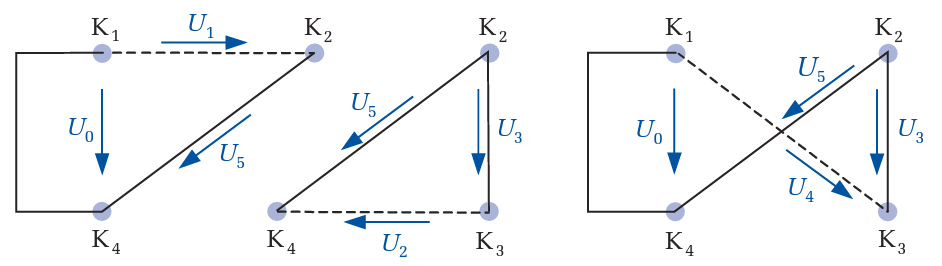
\includegraphics[scale=0.6]{../img/III/IIIjj}}
\centering
\caption{Aufstellung der Maschengleichungen beim vollständigen Baum.}
\label{fig_IIIjj}
\end{figure}
Die drei in der \textbf{\textit{Abbildung \ref{fig_IIIjj}}} dargestellten Maschen führen auf die Gleichungen
\begin{equation}
\boxed{
\begin{array}{lllllll}
M_1:&U_1&&&&+U_5&=U_0\\    
M_2:&&U_2&+U_3&&-U_5&=0\\    
M_3:&&&-U_3&+U_4&+U_5&=U_0\\    
\end{array}
}
\end{equation}
Zusammen mit den Ohm'schen Beziehungn an den fünf Widerständen liegen jetzt elf Gleichungen zur Bestimmung aller unbekannten Ströme und Spannungen in dem Netzwerk vor. Zur Reduzierung des Gleichungssystems können die Zweigspannungen mithilfe des Ohm'schen Gesetzes durch die Zweigströme ersetzt werden. Mit den Knoten- und den Maschengleichungen liegen jetzt genau $z=6$ Bestimmungsgleichungen vor, aus denen alle zweigströme $I_0$ bis $I_5$ eindeutig berechnet werden können. Mit den Strömen sind auch alle Zweigspannungen bekannt und das Problem ist vollständig gelöst.
\begin{equation}
\boxed{
\begin{array}{lllllll}
M_1:&R_1I_1&&&&+R_5I_5&=U_0\\    
M_2:&&R_2I_2&+R_3I_3&&-R_5I_5&=0\\    
M_3:&&&-R_3I_3&+R_4I_4&+R_5I_5&=U_0\\    
\end{array}
}
\end{equation} 
Die zweite Methode wird als \textbf{Auftrennung der Maschen} bezeichnet. Die Vorgehensweise ist relativ einfach. Man wählt einen beliebigen Maschenumlauf und stellt die zugehörige Gleichung auf. Diese Masche wird jetzt an einem beliebigen Zweig aufgetrennt, der in den folgenden Maschen nicht mehr verwendet werden darf. 
\begin{figure}[H]
\frame{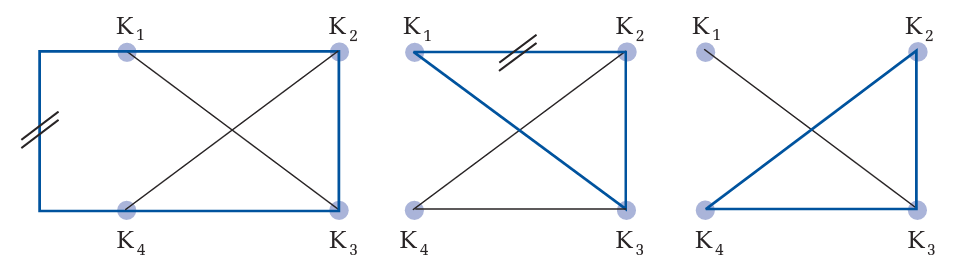
\includegraphics[scale=0.6]{../img/III/IIIkk}}
\centering
\caption{Auftrennung der Maschen.}
\label{fig_IIIkk}
\end{figure}
\noindent Ausgehend von dem verbleibenden Netzwerk stellt man wieder eine Maschengleichung auf und trennt dieese Masche ebenfalls auf. Die fortgesetzte Anwendung dieser Methode liefert ebenfalls die benötigten $m=z-\left(k-1\right)$ Gleichungen. Die lineare Unabhängigkeit dieser Gleichungen ist leicht einzusehen. Beginnt man die Überprüfung bei der zuletzt aufgestellten Beziehung, dann erkennt man unmittelbar, dass die jeweils zuvor aufgestellte Gleichung einen weiteren Zweig enthält, der nachher nicht mehr verwendet wurde, d.h. jede Gleichung ist infolge der Maschenauftrennung zwangsläufig linear unabhängig von den nachfolgend aufgestellten Gleichungen.